\chapter{\textit{Bot} Educacional para Metodologias Ativas em Ambientes
Virtuais}
\label{cap:bot}

% Usar o graphicspath para buscar figuras no subdiretório figuras
\graphicspath{\currfiledir/figuras/}

Este capítulo apresenta a concepção do \textit{bot} educacional desenvolvido
neste trabalho, sua arquitetura funcional e como ele se integra ao ambiente de
ensino remoto para facilitar metodologias ativas. Para ilustrar a aplicação
prática, utilizaremos um exemplo concreto baseado em uma aula de programação da
disciplina CI1055 (Algoritmos e Estruturas de Dados I) do DINF da UFPR
\cite{ufpr2021ci1055}.

\section{Visão Conceitual da Aplicação}
\label{sec:visao}

O \textit{bot} educacional proposto foi concebido como um mediador de interações
em ambientes virtuais de aprendizagem, especificamente voltado para facilitar a
implementação de metodologias ativas durante sessões de ensino remoto. O sistema
atua como uma ponte entre professor e alunos, promovendo trocas mais naturais de
informações e \textit{feedback}.

A Figura a seguir ilustra o modelo conceitual de interação entre os
participantes do processo educacional mediado pelo \textit{bot}:

\begin{figure}[htb]
\centering
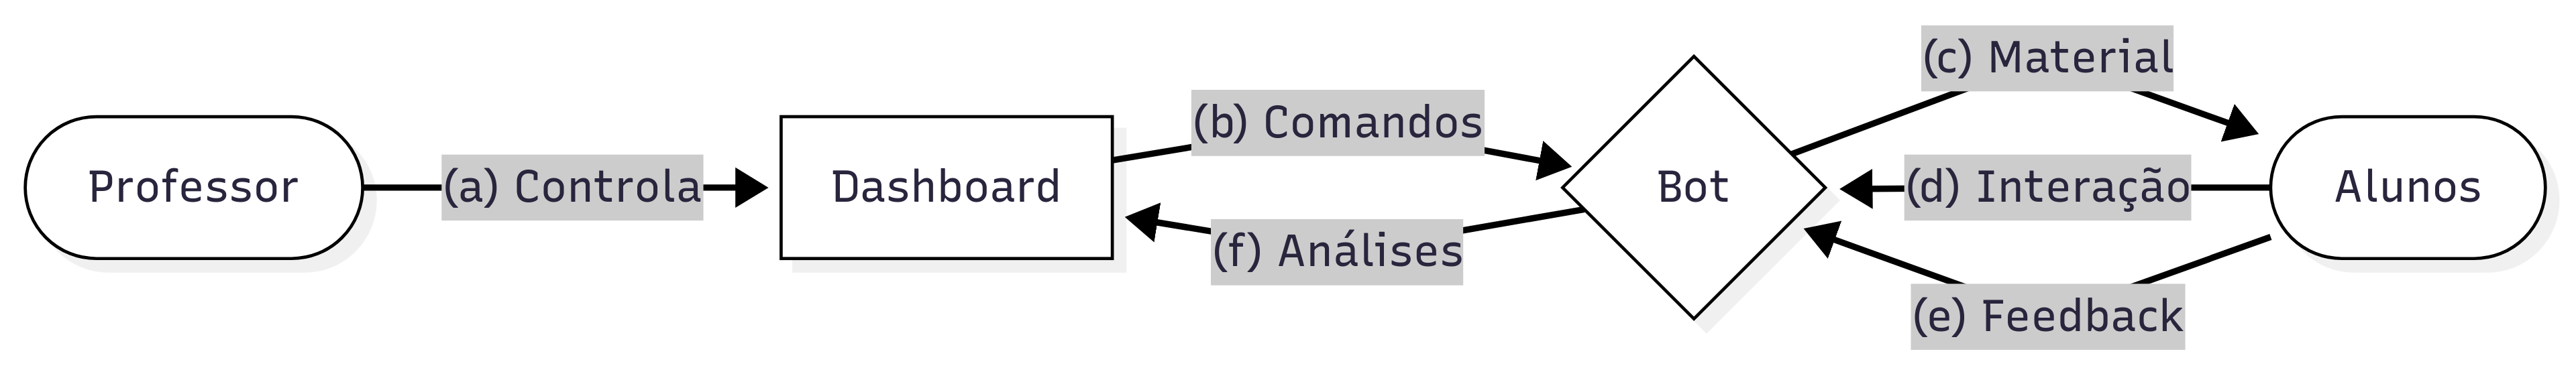
\includegraphics[width=16cm]{modelo-interacao.png}
\caption{Fluxo de interações no ambiente educacional virtual mediado pelo
\textit{bot}. A figura mostra um diagrama com o professor à esquerda, o
\textit{dashboard} do professor como interface de controle, o \textit{bot}
educacional ao centro, e os alunos à direita, ilustrando os fluxos de
comunicação: (a) professor controlando a aula via \textit{dashboard}, (b)
\textit{dashboard} enviando comandos ao \textit{bot}, (c) \textit{bot} 
processando e disponibilizando o material para os alunos, (d) alunos interagindo
com o conteúdo, (e) \textit{bot} coletando \textit{feedback} dos alunos, e (f)
\textit{bot} fornecendo análises em tempo real ao professor através do
\textit{dashboard}.} 
\label{fig:modelo-interacao}
\end{figure}

O modelo de interação implementado neste trabalho fundamenta-se nos três
princípios para interação mediada por \textit{bots} na educação discutidos na
Seção \ref{subsec:principios}: comunicação multidirecional, engajamento ativo e
adaptação contextual. Estes princípios nortearam todo o processo de
\textit{design} e desenvolvimento da solução, garantindo que o \textit{bot}
efetivamente contribua para a implementação de metodologias ativas no ambiente
virtual.

\section{Integração com o Ambiente Educacional}
\label{sec:integracao}

O \textit{bot} foi projetado para se integrar ao Discord, pelos motivos
discutidos na Seção \ref{sec:ferramentas}. A integração sutil com o ambiente
educacional, refere-se à capacidade do \textit{bot} de participar do processo
educacional sem causar rupturas no fluxo natural da aula ou exigir mudanças
drásticas nas práticas pedagógicas já estabelecidas. Essa sutileza manifesta-se
em três dimensões:

\begin{enumerate}
\item \textbf{Presença não-intrusiva}: O \textit{bot} não interrompe a condução
da aula, apenas complementa as atividades quando solicitado ou programado.
\item \textbf{Curva de aprendizado reduzida}: Professores e alunos não precisam
dominar ferramentas complexas, pois as interações ocorrem através de comandos
intuitivos e reações simples.
\item \textbf{Flexibilidade metodológica}: O sistema adapta-se a diferentes
estilos de ensino, não impondo uma abordagem pedagógica específica.
\end{enumerate}

Para materializar esta integração, o sistema também disponibiliza um
\textit{dashboard} específico para uso do professor, como visto em
\ref{subsec:dashboards}, que permite o controle da aula de forma centralizada e
intuitiva, sem a necessidade de comandos complexos ou interrupções no fluxo de
comunicação, como será detalhado na seção \ref{subsec:dashboard}.

\subsection{\textit{Dashboard} do Professor}
\label{subsec:dashboard}

Um elemento chave do sistema é o \textit{dashboard} exclusivo para o professor,
que permite controlar o fluxo da aula sem a necessidade de inserir comandos no
\textit{chat} principal. Este \textit{dashboard} é apresentado como uma
interface web segura, acessível apenas pelo professor, que se comunica com o
\textit{bot} em tempo real. Esta abordagem está diretamente alinhada com o
objetivo de proporcionar uma integração não-invasiva ao fluxo de trabalho
docente, conforme estabelecido na Seção \ref{sec:objetivos} do Capítulo
\ref{cap:revisao}. Através dele, o professor pode:

\begin{itemize}
\item Visualizar estatísticas de engajamento dos alunos em tempo real
\item Controlar a apresentação de slides e materiais didáticos
\item Receber alertas sobre dúvidas e dificuldades dos alunos
\item Lançar atividades interativas e acompanhar seu progresso
\item Obter relatórios detalhados sobre o desempenho da turma
\end{itemize}

Esta abordagem permite que o professor mantenha o controle pedagógico da aula
sem interrupções no fluxo da comunicação, enquanto os alunos interagem
diretamente com o \textit{bot} através de \textit{slash commands} e reações no
ambiente do Discord.

\section{Recursos para Promoção de Metodologias Ativas}
\label{sec:recursos}

O \textit{bot} implementa diversos recursos específicos para viabilizar
metodologias ativas em ambiente remoto. Na seção \ref{subsec:feedback} é
apresentado mecanismos de \textit{feedback} em tempo real que permitem ao
professor avaliar continuamente a compreensão dos alunos, a
\ref{subsec:colaboracao} aborda ferramentas para atividades colaborativas que
incentivam a interação entre os estudantes, e por fim \ref{subsec:pbl} trata das
funcionalidades específicas para aprendizagem baseada em problemas que estimulam
o raciocínio crítico e a resolução de situações práticas.

\subsection{\textit{Feedback} em Tempo Real}
\label{subsec:feedback}

Um dos principais desafios do ensino remoto é perceber as reações dos alunos. O
\textit{bot} permite que os estudantes expressem sua compreensão ou dúvidas
durante a explanação, sem interromper o fluxo da aula, através de:

\begin{itemize}
\item \textbf{Barômetro de compreensão}: Interface visual que agregada as
reações dos alunos
\item \textbf{Alertas de dificuldade}: Notificação ao professor quando um número
significativo de alunos indica não compreender um tópico
\item \textbf{Dúvidas anônimas}: Permite que alunos enviem questões sem
exposição pública
\end{itemize}

\subsection{Atividades Colaborativas}
\label{subsec:colaboracao}

Para fomentar a aprendizagem entre pares, o \textit{bot} oferece:

\begin{itemize}
\item \textbf{Grupos dinâmicos}: Formação automática de equipes para discussão
de tópicos específicos
\item \textbf{Compartilhamento facilitado}: Interface para troca de soluções e
ideias entre alunos
\item \textbf{Revisão coletiva}: Sistema para avaliação colaborativa de
respostas
\end{itemize}

\subsection{Aprendizagem Baseada em Problemas}
\label{subsec:pbl}

A aprendizagem baseada em problemas (vide Seção \ref{cap:intro}) envolve vários
elementos que podem ser incluídos em nosso aplicativo. Dentre esses elementos,
incluímos os seguintes, por serem os mais simples de se implementar:

\begin{itemize}
\item \textbf{Desafios temporizados}: Problemas com tempo definido para
resolução
\item \textbf{Pistas progressivas}: Sugestões que são liberadas gradualmente
durante a resolução
\item \textbf{Compilação e execução de código}: Para disciplinas de programação,
execução segura de códigos submetidos pelos alunos
\end{itemize}

\section{Exemplo Prático: Aula de Comandos de Repetição}
\label{sec:exemplo}

Para ilustrar a aplicação concreta do \textit{bot} em um contexto educacional
real, apresentamos a seguir um cenário baseado em uma aula da disciplina CI1055
- Algoritmos e Estruturas de Dados I, ministrada no Departamento de Informática
da UFPR. O exemplo demonstra como o \textit{bot} auxilia o professor durante uma
aula sobre "Comandos de Repetição" em Pascal. Nas próximas seções, detalharemos
as etapas de preparação da aula pelo professor e as interações que ocorrem
durante a sessão síncrona, evidenciando como os recursos do \textit{bot}
facilitam a implementação das metodologias ativas.

\subsection{Preparação da Aula}
\label{subsec:preparacao}

Antes da aula, o professor utiliza o \textit{dashboard} para preparar o material
didático:

\begin{lstlisting}[
  basicstyle=\ttfamily\footnotesize,
  backgroundcolor=\color{gray!10},
  breaklines=true,
  captionpos=b,
  commentstyle=\color{green!50!black},
  frame=single,
  keywordstyle=\color{blue},
  numbers=left,
  numbersep=5pt,
  numberstyle=\tiny\color{gray},
  stringstyle=\color{red},
  showstringspaces=false,
  tabsize=2
]
[(*@\textit{Dashboard}@*) do Professor]
> Criar Nova Aula
Título: "Comandos de Repetição em Pascal"
Descrição: "Introdução aos comandos de repetição em Pascal com foco no comando while"
Tópicos: "Loops", "Comando while", "Repetição", "Pascal"

> Adicionar Conteúdo
[Título] "Objetivos da aula"
[Conteúdo] "Introduzir conceitos de repetição, apresentar o comando while, 
           resolver exemplos práticos"
[Tipo] Slide

> Adicionar Conteúdo
[Título] "Exemplo inicial: imprimir números de 1 a 5"
[Conteúdo] 
```
program imprimir_de_1_a_5;
begin
  writeln(1);
  writeln(2);
  writeln(3);
  writeln(4);
  writeln(5);
end.
```
[Tipo] Código Pascal

> Configurar Quiz
[Pergunta] "Ao incrementar uma variável dentro de um loop while, 
           qual operação utilizamos em Pascal?"
[Opções] 
- "i := i + 1" (CORRETA)
- "i++"
- "i += 1"
- "increment(i)"
[Tempo] 60 segundos
\end{lstlisting}

O sistema confirma a criação da aula e fornece um código de acesso para os alunos.

\subsection{Interação Durante a Aula}
\label{subsec:interacao}

Durante a aula síncrona, as seguintes interações ocorrem:

\begin{lstlisting}[
  basicstyle=\ttfamily\footnotesize,
  backgroundcolor=\color{gray!10},
  breaklines=true,
  captionpos=b,
  commentstyle=\color{green!50!black},
  frame=single,
  keywordstyle=\color{blue},
  numbers=left,
  numbersep=5pt,
  numberstyle=\tiny\color{gray},
  stringstyle=\color{red},
  showstringspaces=false,
  tabsize=2
]
[(*@\textit{Dashboard}@*) do Professor]
> Iniciar Aula "Comandos de Repetição em Pascal"
Sistema: Aula iniciada. Os alunos podem acessar usando o código #AED1-2310.

> Mostrar Slide 1
Sistema: Exibindo "Objetivos da aula" para todos os participantes.

[Discord - Canal da Aula]
Bot: @everyone O professor iniciou a aula "Comandos de Repetição em Pascal". 
     Use (*@\textit{/participar}@*) para confirmar sua presença.

[Vários alunos utilizam o comando (*@\textit{/participar}@*)]

Professor [no canal de voz]: Vamos começar entendendo por que precisamos de comandos 
                             de repetição. Observem este exemplo inicial no canal.

[(*@\textit{Dashboard}@*) do Professor]
> Mostrar Código "Exemplo inicial"
Sistema: Código exibido no canal #exemplos-de-codigo.

[Discord - Canal #exemplos-de-codigo]
Bot: 
```pascal
program imprimir_de_1_a_5;
begin
  writeln(1);
  writeln(2);
  writeln(3);
  writeln(4);
  writeln(5);
end.
```
Para testar este código, utilize /executar exemplo1

[(*@\textit{Dashboard}@*) do Professor]
> Iniciar Discussão
[Pergunta] "Qual o problema desta abordagem se quisermos imprimir de 1 até 1000?"

[Discord - Canal da Aula]
Bot: DISCUSSÃO: Qual o problema desta abordagem se quisermos imprimir de 1 até 1000?
     Use (*@\textit{/responder}@*) para participar da discussão.

Aluno1: (*@\textit{/responder}@*) Teríamos que escrever mil linhas de código!
Aluno2: (*@\textit{/responder}@*) Código muito repetitivo e difícil de manter.

[(*@\textit{Dashboard}@*) do Professor - Painel de Engajamento]
Status: 15/23 alunos responderam
Participação ativa: 65%
Respostas mais comuns: "código repetitivo" (60%), "muitas linhas" (27%)

[Alguns alunos usam reações no Discord]
[5 alunos reagem com "joinha" (entendi)]
[2 alunos reagem com "?" (tenho dúvida)]

[(*@\textit{Dashboard}@*) do Professor - Alertas]
ATENÇÃO 2 alunos indicaram dúvidas sobre o conceito atual.
Recomendação: Revisitar o conceito com uma abordagem alternativa.

Professor [no canal de voz]: Estou vendo que temos algumas dúvidas. 
                             Vamos revisitar o conceito de forma diferente.

[(*@\textit{Dashboard}@*) do Professor]
> Mostrar Exemplo Interativo
[Título] "Loop while básico"
[Código]
```pascal
program exemplo;
var i: integer;
begin
  i := 1;
  while i <= 5 do
  begin
    writeln(i);
    i := i + 1;
  end;
end.
```
[Opções] Ativar execução por alunos

[Discord - Canal #exemplos-de-codigo]
Bot: EXEMPLO INTERATIVO: Loop while básico
```pascal
program exemplo;
var i: integer;
begin
  i := 1;
  while i <= 5 do
  begin
    writeln(i);
    i := i + 1;
  end;
end.
```
Use /executar para ver o resultado deste código.

Aluno5: /executar
Bot: 
```
1
2
3
4
5
```

Aluno8: /duvida O que acontece se eu esquecer de incrementar i dentro do loop?
Bot: @Professor Dúvida enviada anonimamente: "O que acontece se eu esquecer de incrementar i dentro do loop?"

[(*@\textit{Dashboard}@*) do Professor]
> Responder Dúvida
[Criar Exemplo] "Loop infinito"
```pascal
program loop_infinito;
var i: integer;
begin
  i := 1;
  while i <= 5 do
  begin
    writeln(i);
    // i não é incrementado
  end;
end.
```

[Discord - Canal #exemplos-de-codigo]
Bot: Resposta à dúvida: O que acontece se esquecer de incrementar i
```pascal
program loop_infinito;
var i: integer;
begin
  i := 1;
  while i <= 5 do
  begin
    writeln(i);
    // i não é incrementado
  end;
end.
```
Aviso: O código acima contém um loop infinito. A execução seria interrompida após 
repetir o mesmo valor várias vezes:
```
1
1
1
1
...
```

[(*@\textit{Dashboard}@*) do Professor]
> Criar Desafio
[Título] "Números pares"
[Descrição] "Escreva um programa que leia um número n e imprima todos os números pares de 2 até n"
[Tempo] 10 minutos
[Testes Automáticos] 
- Entrada: "10" | Saída esperada: "2 4 6 8 10"
- Entrada: "7" | Saída esperada: "2 4 6"

[Discord - Canal #desafios]
Bot: NOVO DESAFIO: Números pares
Escreva um programa que leia um número n e imprima todos os números pares de 2 até n.
Tempo: 10 minutos
Use /iniciar-desafio para começar a resolver.

[Vários alunos utilizam o comando /iniciar-desafio, recebendo acesso a canais privados para resolver o problema]

[(*@\textit{Dashboard}@*) do Professor - Monitor de Progresso]
15/23 alunos iniciaram o desafio
8/23 já submeteram soluções
6/23 passaram em todos os testes

[Após o tempo definido]
[(*@\textit{Dashboard}@*) do Professor]
> Encerrar Desafio
> Compartilhar Solução Anônima [ID: 3]

[Discord - Canal #desafios]
Bot: O tempo para o desafio "Números pares" encerrou!
Estatísticas:
- 19/23 alunos participaram
- 15/19 completaram o desafio com sucesso

Solução compartilhada (anônima):
```pascal
program numeros_pares;
var i, n: integer;
begin
  read(n);
  i := 2;
  while i <= n do
  begin
    writeln(i);
    i := i + 2;
  end;
end.
```

[(*@\textit{Dashboard}@*) do Professor]
> Encerrar Aula
> Gerar Relatório

[Discord - Canal da Aula]
Bot: Esta aula foi encerrada. Um resumo das atividades foi enviado ao professor.
     Todo o material continua disponível para consulta nos canais respectivos.

[(*@\textit{E-mail}@*) do Professor - Relatório Automático]
Resumo da aula: "Comandos de Repetição em Pascal"
- Participação: 23/25 alunos ativos (92%)
- Média de interações por aluno: 7.2
- Tópicos com mais dúvidas: "loop infinito" (5 menções), "incremento de variáveis" (3 menções)
- Desafio "Números pares": 19/23 participaram, 15/19 completaram com sucesso
- Alunos com participação abaixo do esperado: 2 (lista anexa)
- Recomendação: Reforçar o conceito de incremento de variáveis na próxima aula
\end{lstlisting}
